\documentclass[french]{article}
\usepackage[utf8]{inputenc}
\usepackage[T1]{fontenc}

\usepackage{natbib}
\usepackage[vmargin=3cm,left=4cm,right=4cm]{geometry}

\usepackage{babel}

\usepackage{graphicx}
\usepackage{caption} 
\captionsetup{justification=centering}
\usepackage{subcaption}
% \usepackage{hyperref}
\usepackage[hidelinks]{hyperref}

\begin{document}

%###############################################
\begin{titlepage}

\newcommand{\HRule}{\rule{\linewidth}{0.5mm}} % Defines a new command for the horizontal lines, change thickness here

\center % Center everything on the page
 
%----------------------------------------------------------------------------------------
%	Section Titre
%----------------------------------------------------------------------------------------
\HRule \\[0.4cm]
\vspace{1cm}
{ \huge \bfseries Trombinoscope}\\ % Title of your document
\vspace{1cm}
\HRule \\[1cm]
 
%----------------------------------------------------------------------------------------
%	Section auteur
%----------------------------------------------------------------------------------------
\vspace{1cm}

\Large \today

\vspace{3cm}

\begin{minipage}{0.4\textwidth}
\begin{center}
\Large \textbf{Auteurs :}\\
\vspace{0.5cm}
Nathan \textsc{Faudeil} \\
Quentin \textsc{Guichoux}\\
Fabio \textsc{Cassiano}
\end{center}
\end{minipage}

\vspace{5cm}

\begin{figure}[!ht]
    %\hspace*{-0.5cm}
	
\includegraphics[height=0.1\columnwidth]{Image/logo/logo_simplon.png}
	\hspace*{0.5cm}
	
\includegraphics[height=0.12\columnwidth]{Image/logo/logo_Isen.png}
	\hspace*{0.5cm}
	
\includegraphics[height=0.1\columnwidth]{Image/logo/logo_microsoft.jpg}
\end{figure}

\vfill

\end{titlepage}

\newpage

\tableofcontents

\newpage

\section{Arbre de décision}

\begin{figure}[!htbp]
    \centering
    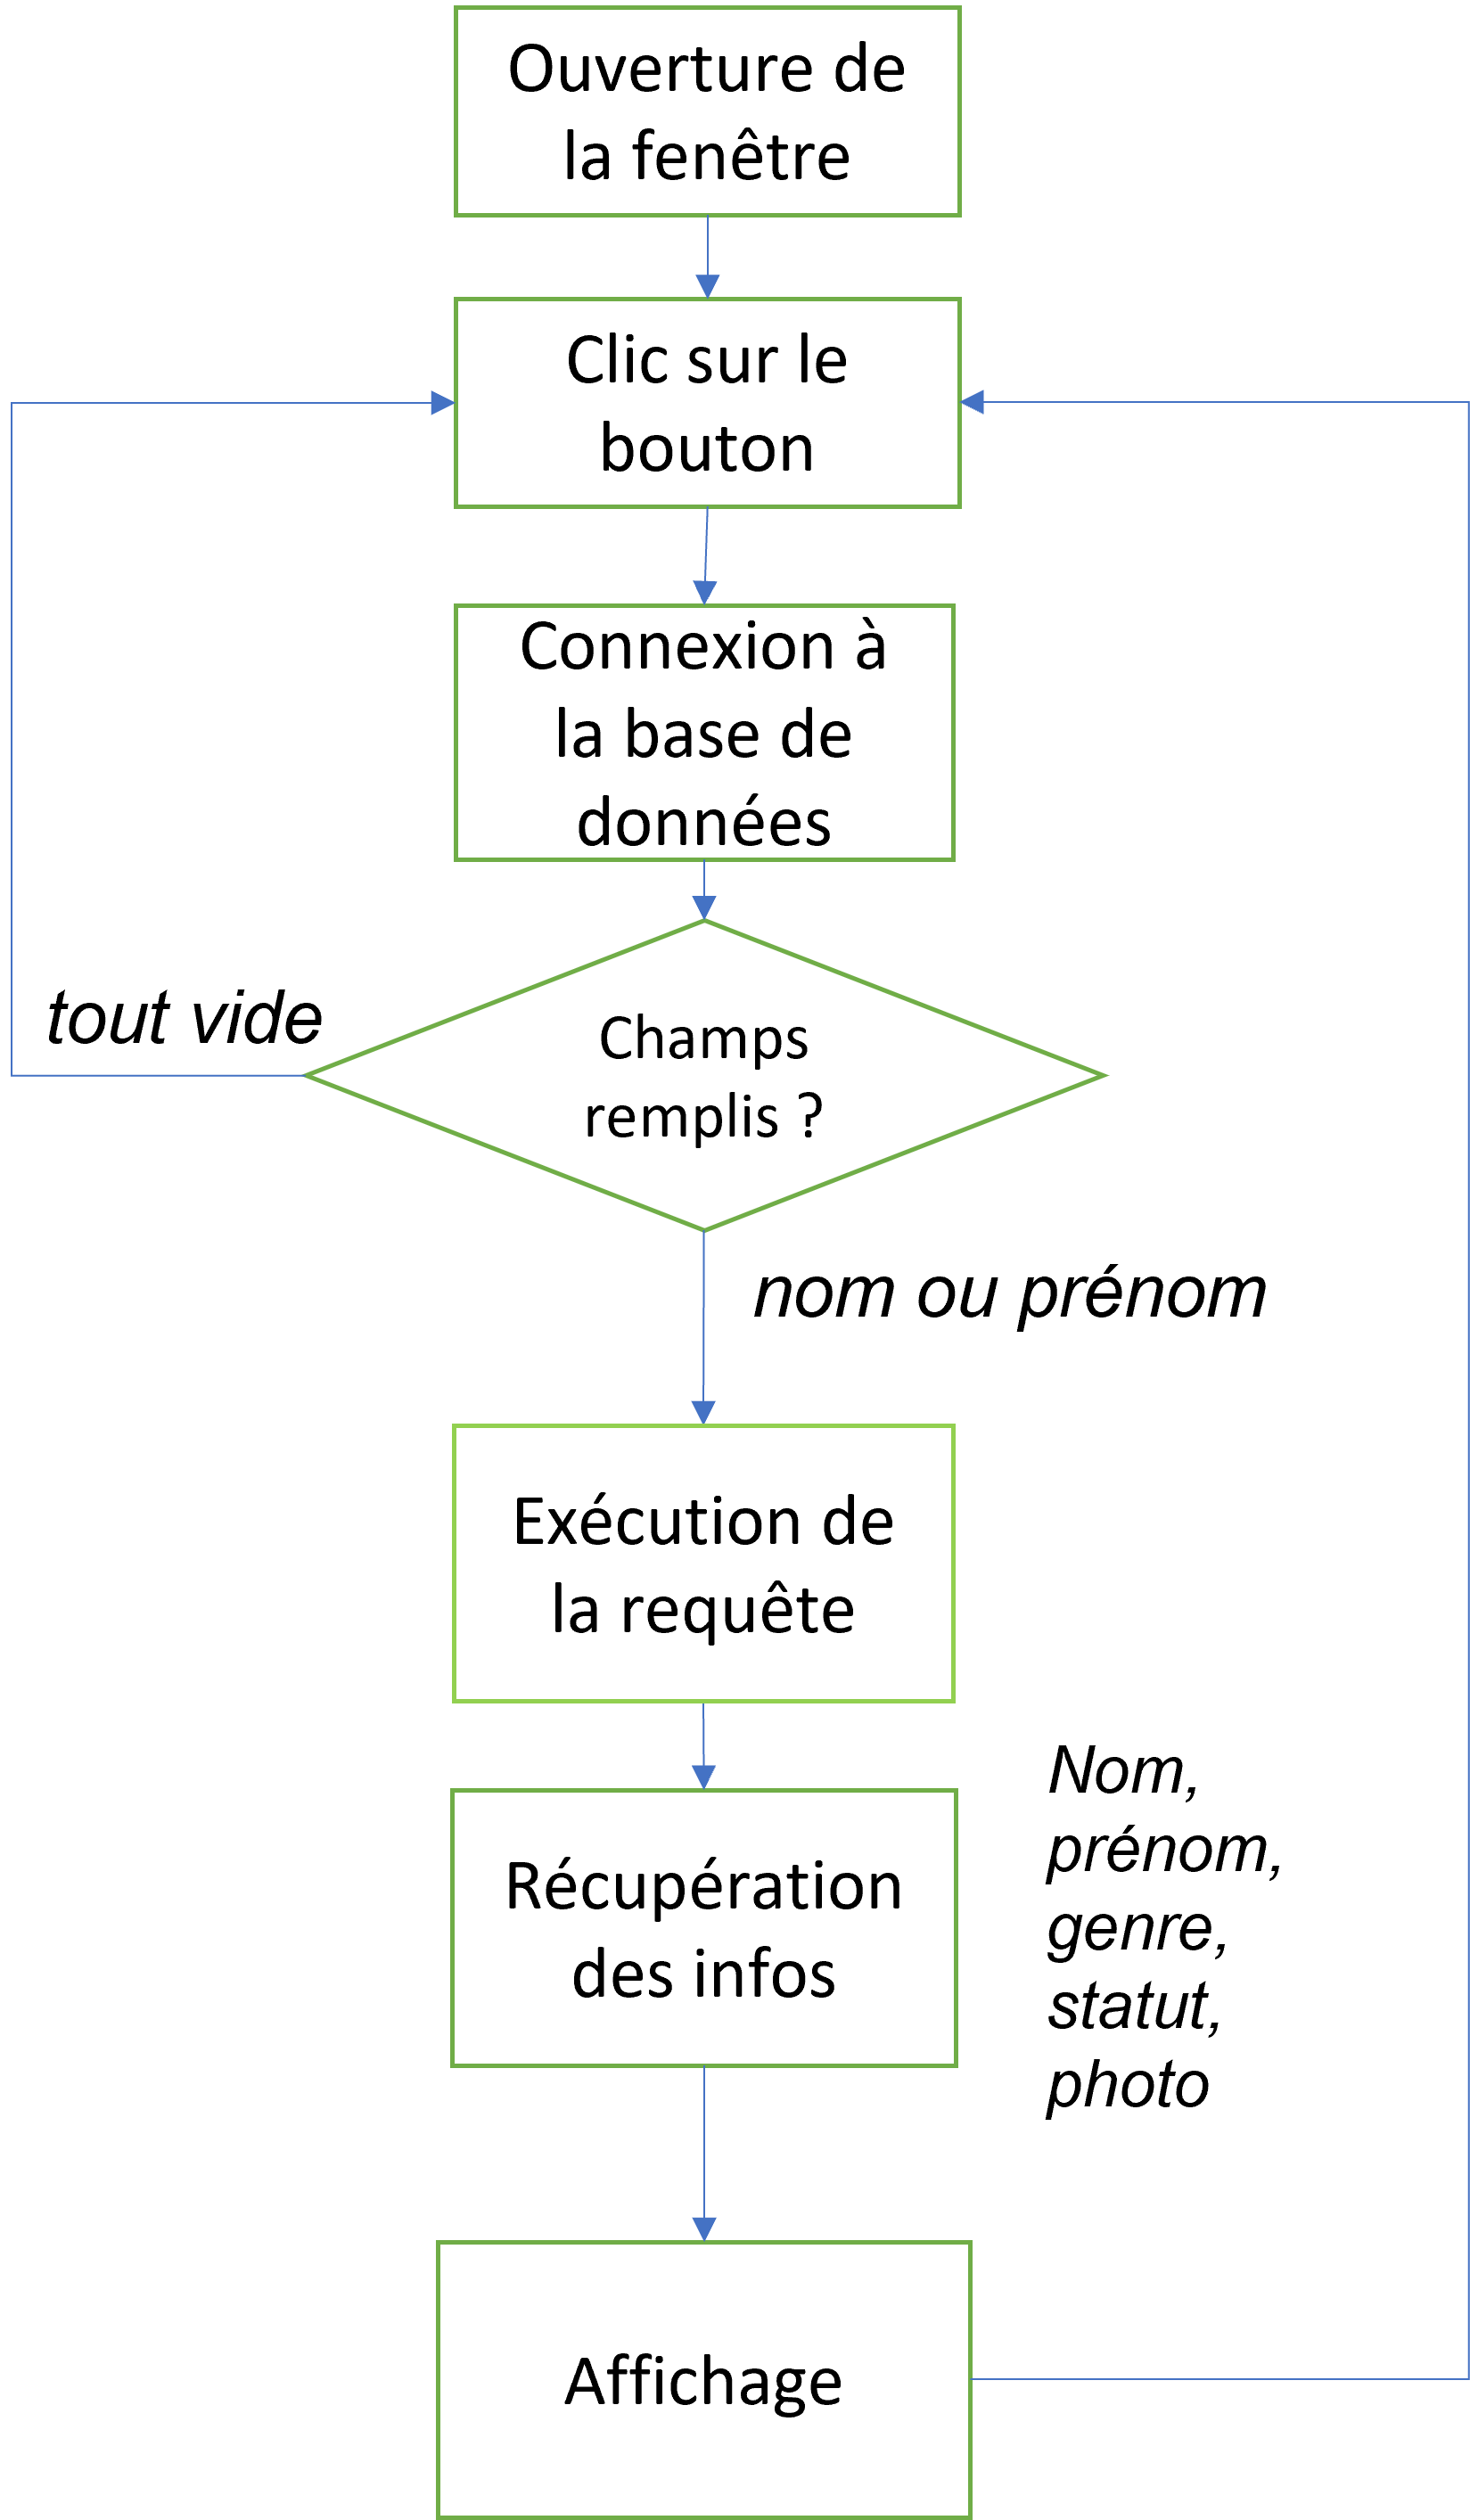
\includegraphics[width=.7\textwidth]{Image/arbre_decision.png}
    \caption{Arbre de décisions de l'application trombinoscope. \\ \textit{Les champs de saisie correspondent au nom, prénom, genre, statut, photo et l'interrogation de la base de données jusqu'à l'affichage se fait de manière invisible pour l'utilisateur}}
    \label{fig:arbre}
\end{figure}

\newpage

\section{Guide utilisateur}
\subsection{Captures d'écran de la solution}
\begin{figure}[!htbp]
    \begin{subfigure}[b]{\textwidth}
        \centering
        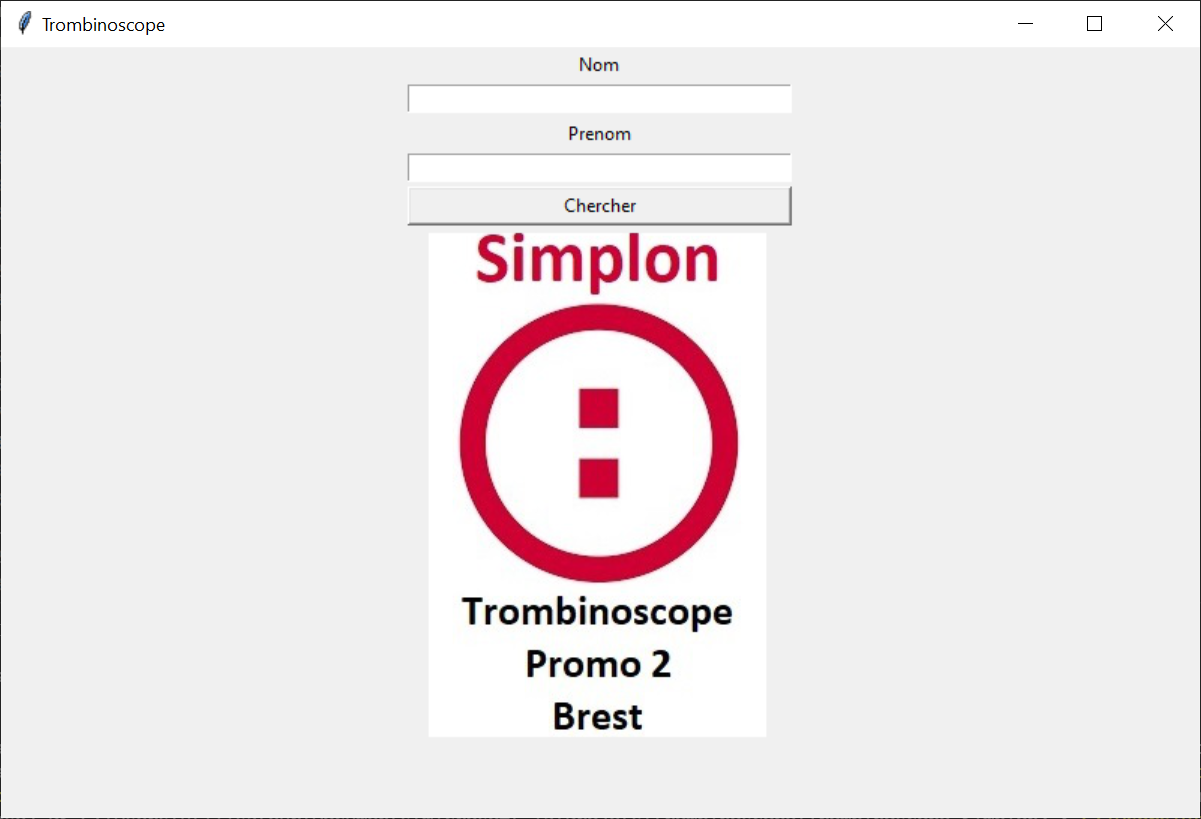
\includegraphics[scale=0.5]{Image/main_window.PNG}
        \caption{Fenêtre de démarrage}
        \label{fig:mainwindow}
    \end{subfigure}
    \vfill
    \begin{subfigure}[b]{\textwidth}
        \centering
        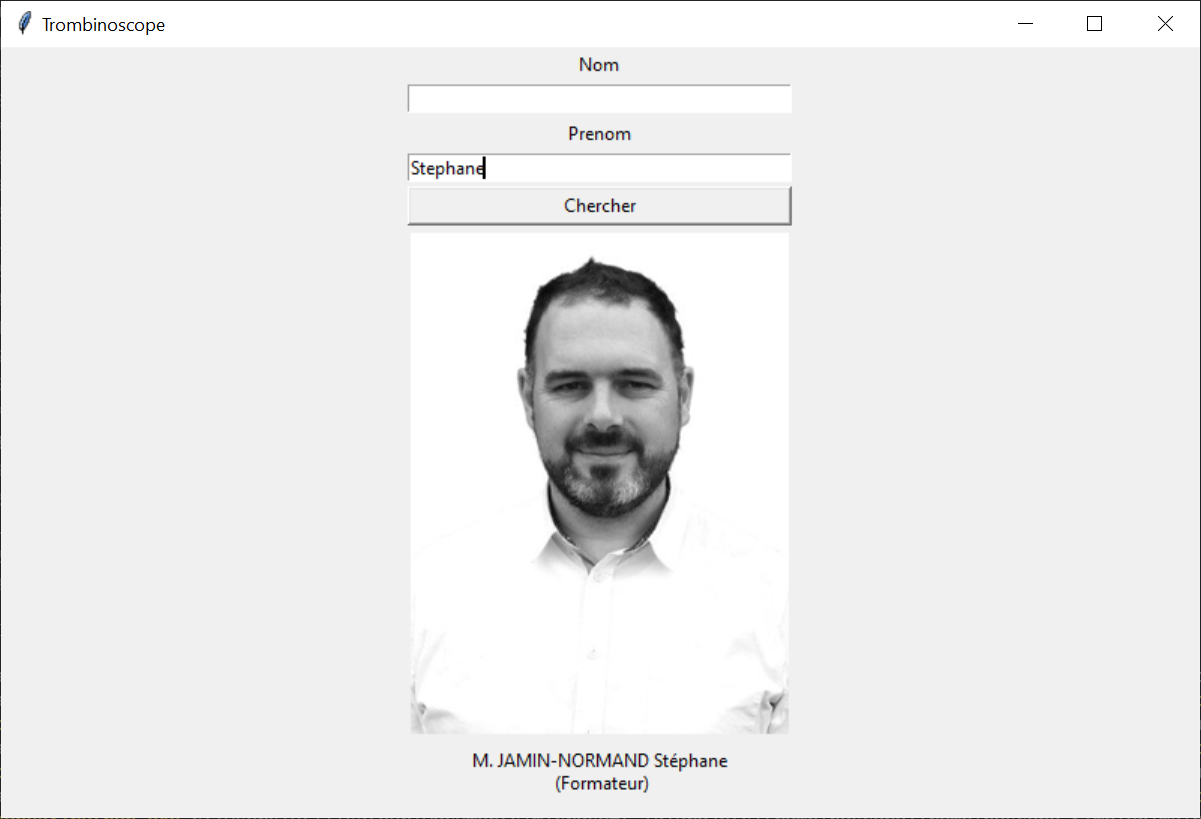
\includegraphics[scale=0.5]{Image/window_reseach.PNG}
        \caption{Recherche d'une personne par le prénom}
        \label{fig:tb_recherche}
    \end{subfigure}
    \caption{Interface de l'application trombinoscope}
\end{figure}

\subsection{Explication du fonctionnement}

\subsubsection{\textit{Version 1.0}}
Le trombinoscope que nous avons créé fonctionne par la recherche du \textbf{\textit{Nom}} ou du \textbf{\textit{Prénom}} de la personne. Pour se faire un champ de saisie est mis à disposition de l'utilisateur pour chacun de ces deux paramètres (Fig. \ref{fig:mainwindow}). Le bouton \textbf{recherche} permet ensuite d'activer une requête SQL qui utilise les champs remplis pour retrouver dans la base de données la personne correspondante et de récupérer les informations suivantes :
\begin{enumerate}
    \item Nom de la personne
    \item Prénom de la personne
    \item Photo associée
    \item Genre associé (M., Mme., Autre)
    \item Statut associé (Étudiant P2, Formateur, Chargé de Formation)\\
\end{enumerate}

\noindent Ces informations sont ensuite renvoyées sur l'interface utilisateur, en affichant la photo associée (Fig. \ref{fig:tb_recherche}), puis les informations de la personne sous la forme : 
\begin{center}
    \textit{Genre Nom Prénom (Statut)}\\
\end{center}

\subsubsection{\textit{Version 2.0}}

La seconde version du trombinoscope a subit une légère modification de l'interface. La partie recherche se trouve maintenant à gauche de la partie affichage.\\

Il est maintenant possible de réaliser une recherche par le genre ou le statut. Cette fonctionnalité se matérialise par deux \textit{listebox} en dessous du champ prénom.\\

Coté affichage il est maintenant possible d'afficher plusieurs photo ainsi que les informations associés.\\

\begin{figure}[!htbp]
    \centering
    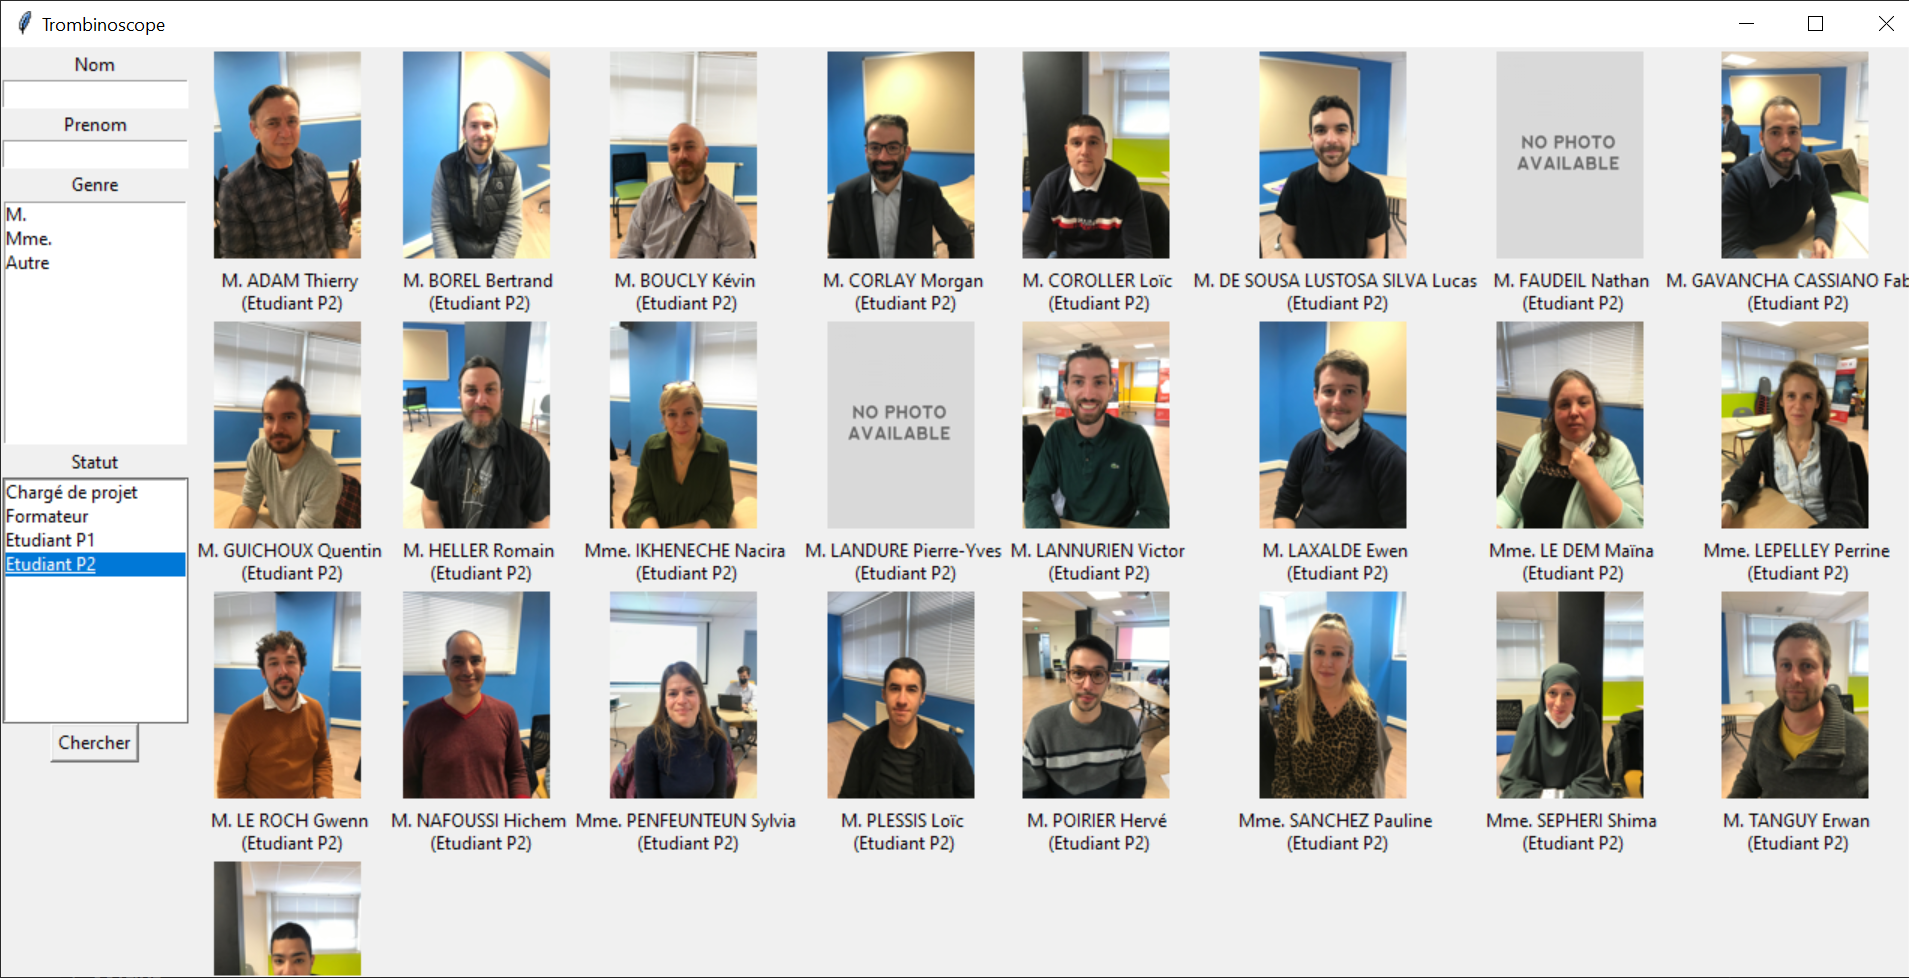
\includegraphics[width=\textwidth]{Image/trombinoscope_v2.PNG}
    \caption{Trombinoscope version 2.0 \\ Représentation de l'interface du trombinoscope version 2.0 avec la recherche de toute la promotion 2 (Les \textit{Breizhmeiz})}
    \label{fig:tromb_v2}
\end{figure}


\section{Présentation du schéma de la base de données}

\begin{figure}[!htbp]
    \centering
    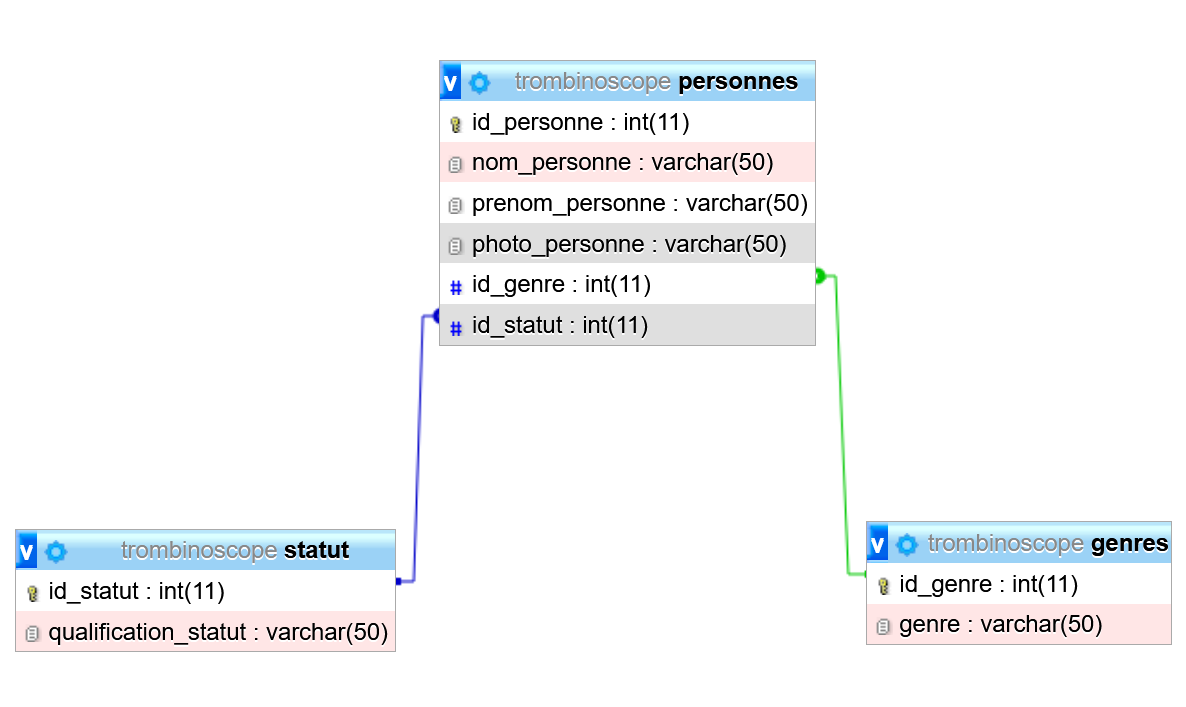
\includegraphics[width=\textwidth]{Image/db_mysql.png}
    \caption{Schéma de la base de données trombinoscope}
    \label{fig:db}
\end{figure}

\subsection{Les difficultés}
    L'objectif de la base de données était de créer un document contenant les informations des différentes personnes présentes à la formation. 
    
    La création du schéma relationnel de la base de données n'a pas posé de réels problèmes, la base étant simple et de petite taille.
\subsection{Les solutions}
    Le choix de renseigner le genre et le statut de la personne à rendu obligatoire la création de plusieurs tables. 
    Une personne ne pouvant avoir qu'un seul genre et qu'un seul statut, des tables intermédiaires auraient été superflues, et nous avons donc donc créé trois tables :
    \begin{enumerate}
        \item \textit{Personnes}, contenant les noms, prénoms et identifiants des apprenants et formateurs
        \item \textit{Statut}, contenant les différents rôles qu'une personne peut avoir (apprenant ou formateur)
        \item \textit{Genres}, contenant les différents genres possibles (M., Mme., autre). Pour lier ces différentes tables, nous avons créé des identifiants dans chacune d'entre-elles, tous mis en clé primaire, puis nous avons rajouté id\_genre et id\_statut en clés étrangères dans la table \textit{Personnes} pour pouvoir accéder à toutes les informations. \\
    \end{enumerate} 
    
    
\section{Présentation du code Python}
\subsection{Les difficultés}
    Nous avons rencontré une difficulté lors de l'affichage des images. En effet, lors de la recherche d'une personne, la photo apparaissait mal centrée dans le cadre dédié à son affichage. 
\subsection{Les solutions}
    Nous voulions afficher les photos au centre du canevas créé à cette fin, afin qu'elles soient centrées. Les dimensions du canevas étaient sous la forme \textit{hauteur/largeur}. Notre erreur résidait dans le fait que nous avions indiqué dans le code que nous voulions projeter le centre de la photo en position (0,0) du canevas. Cela faisait donc apparaître le centre de l'image dans le coin nord/ouest de ce dernier, occasionnant le décalage que nous ne comprenions pas. Une fois l'erreur réalisée, nous avons tout simplement changé la position (0,0) en \textit{(hauteur/2, largeur/2)}, et le problème était réglé. \\  
    
    

\section{Apprentissage}
\subsection{Fabio}
    Pour ma part j'avais déjà quelques notions de SQL en ligne de commande. Grâce à ce projet j'ai pu consolider mes connaissances en création de base de données, et j'ai également pu découvrir l'utilisation de phpmyadmin pour l'administration de base de données avec une interface graphique. Pour Python, j'avais déjà utilisé ce langage pour des traitements scientifiques. Ici j'ai pu découvrir Tkinter, et ainsi la création d'interfaces sous ce langage. Les compétences développées par le biais de ce projet me permettront d'améliorer les futurs projets sur lesquels je travaillerai.
\subsection{Quentin}
    Connaissant déjà relativement bien le SQL et phpmyadmin j'ai surtout pu découvrir de manière plus poussée Python. Avant ce projet, je ne m'en servais que d'une manière assez basique sans trop utiliser de bibliothèques. La découverte de TKinter me permet de mieux utiliser ce langage et de faire de petits projets personnels plus aboutis, et dans l'avenir utiliser ces connaissances en situation professionnelle. 
\subsection{Nathan}
    Au début du projet, je n'avais qu'une compréhension limitée de Python, le reste m'était inconnu. En créant le trombinoscope, j'ai pu découvrir SQL, phpmyadmin, ainsi que l'utilisation de la bibliothèque Tkinter. J'ai surtout eu la chance d'être bien accompagné par mes camarades qui connaissaient davantage cet environnement. L'utilisation générale de tous ces outils n'est bien évidemment pas encore totalement acquise, mais cela m'apparaît moins étranger. Je pense que toutes ces compétences pourront me servir pour mieux cerner les implications liées au domaine de l'intelligence artificielle, pour la suite de la formation mais également pour mon projet professionnel. \\
    
\newpage
\section{Conclusion}
\subsection{Que souhaitez-vous apprendre sur SQL et Python?}
    La question nous semble peut-être encore prématurée, étant donné que nous ne connaissons pas toutes les implications de SQL et Python dans le domaine de l'intelligence artificielle. Le trombinoscope était donc une bonne base de départ dans l'apprentissage de ces outils, nous verrons au travers des autres projets ce qui nous intéresse davantage dans leurs usages. 
\subsection{Quelles évolutions envisagez-vous sur l'application?}
\subsubsection{Version 1.0}
    \noindent Nous avons réfléchi sur plusieurs améliorations du trombinoscope :
    \begin{enumerate}
        \item Faire en sorte que le bouton "rechercher" soit activé par la touche "entrée" du clavier pour accélérer la recherche et ne pas utiliser la souris.
        \item Certaines personnes de la formation ont le même nom de famille où le même prénom. Une amélioration possible serait, lors d'une recherche par nom où prénom, d'afficher la photo des deux personnes en même temps, ce qui n'est pas le cas dans le trombinoscope actuellement. (\textit{Effectif dans la version 2.0}) 
        \item Faire en sorte d'afficher plus de critères de sélection. Par exemple chercher par genre ou par statut, et dans ce cas prévoir une amélioration de l'affichage et une aide à la navigation entre les différents profils. (\textit{Effectif dans la version 2.0}) 
        \item Une interface homme-machine (IHM) plus aboutie et polie pourrait également être une bonne chose. Nos connaissances de TKinter étant limitées, notre interface reste relativement basique. 
        \item En cas d'éventuelle mise en ligne du projet une protection contre les attaques par injection SQL, bien que n'ayant pas de données sensibles ou de connexion, un "nom');DROP TABLE Personne--" serait à éviter. Dans le cadre du projet une protection contre ces attaques n'est pas utile mais pour des projets futurs ou des mise en ligne, il serait utile d'en incorporer une. 
        
    \end{enumerate}
      
\subsubsection{Version 2.0}

\noindent D'autres améliorations ont été ajoutées pour la version 2.0 du trombinoscope :
\begin{enumerate}
    \item Pouvoir effectuer des recherches en combinant les champs. Par exemple, si une femme et un homme avaient le même nom de famille, on pourrait en afficher un seul en sélectionnant le genre associé.
    \item Adapter la taille des photos affichées à l'espace disponible, ainsi que permettre de défiler vers le bas quand les photos sont trop nombreuses. Pour le moment, toutes les photos ont une taille fixe et suffisamment petite pour permettre d'afficher une grande quantité d'image.
\end{enumerate}

\end{document}
